\mysection{Evaluation}

As described in \subsecref{Building the models} the accuracy can be improved by playing around with the training steps and the learning rate. It's a tradeoff between good results and overfitting, so that the model is too specialized on the training set.

The best values for the MobileNet0.5 model are achieved with 700 training steps and a learning rate of 0.007.

For the MobileNet1.0 model it was hard to find really well values. So the best here are 500 training steps and a learning rate of 0.01.

The final Inception model was retrained with 4000 training steps and a learning rate of 0.03.

For all models the \textit{accuracy}- and \textit{cross entropy}-diagram from TensorBoard is depicted in the appendix under \subsecref{TensorBoard - optimal achieved accuracy of the different models} (\figref{MobileNet05-700res} till \figref{AllRes}). Exact these models are now used for further work.\\



In oder to compare the different optimization attempts, a bash script named \textit{eval_label-image.sh} was written. It's placed in the github repository of this project in the directory \textit{code/scripts}. The script takes a choosen set of 20 images (works/Evaluierung/eval_label_image_pics) and calls internally the \textit{label_image.py} script to label them. The images, which partly are very difficult to classify, are picked from both dog datasets mentioned in \subsecref{Dataset}. In an Excel-sheet the results are averaged which is depicted in detail in the appendix under \subsecref{Evaluation of optimization attempts} (\tabref{mobileNet05} till \tabref{inception}) and graphically in \figref{evalAccTime2}.  \\

\begin{figure}[htbp]
\centering
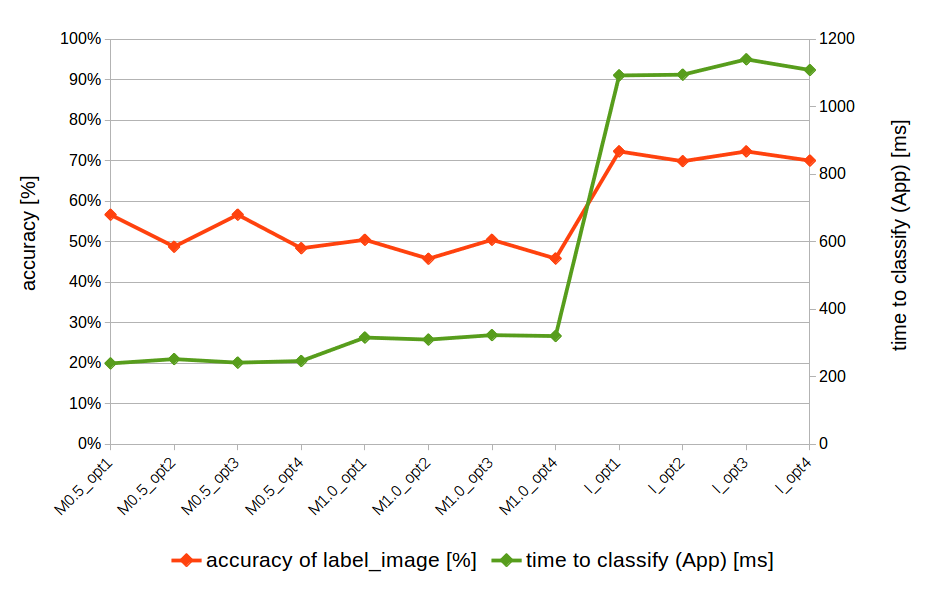
\includegraphics[width=0.9\textwidth]{includes/evalAccTime2}
\caption{Accuracy and time to classify of different optimization attempts}
\label{fig:evalAccTime2}
\end{figure}

Because of the great benefit with the compression (refer to \subsecref{Building the models}) and the fact that the accuracy and the classification time of \textit{opt2} and \textit{opt4} isn't dramatically worser in contrast to the others, these two attempts are a good choice. Looking exactly at the tables, \textit{opt4} is a little bit more accurate, so this is the best one and will be used for further comparisons. \\

For evaluating the different model architectures the last chart (\figref{evalAccTime2}) was represented as a scatter plot, which is shown in \figref{evalAccTime}. So in this plot the upper left corner would be the best tradeoff between accuracy and performance of the mobile app. Thus one of the two MobileNets would be selected. \\

\begin{figure}[htbp]
\centering
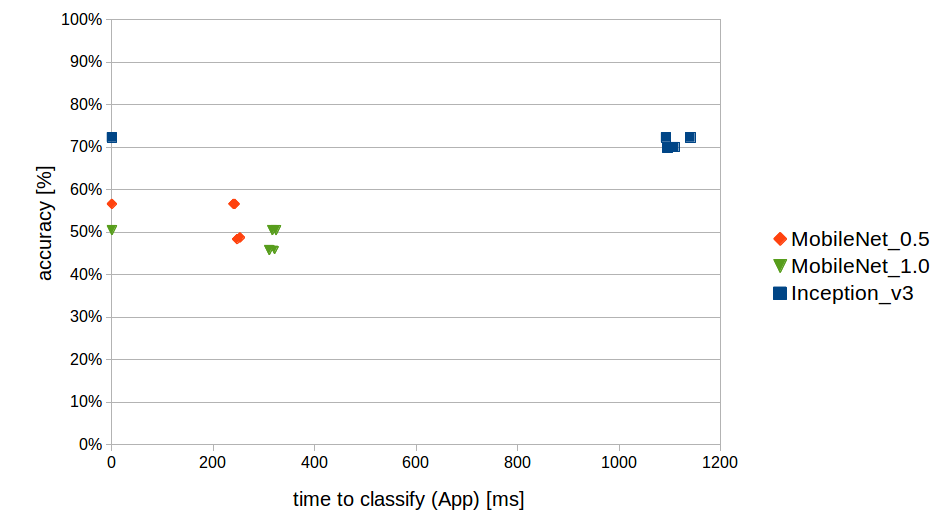
\includegraphics[width=\textwidth]{includes/evalAccTime}
\caption[evalAccTime2]{Accuracy in relation to classification time of different models}
\label{fig:evalAccTime}
\end{figure}




However for a more accurate evaluation of the models, some more facts have to be considered, which is shown in \tabref{finalEval} in numbers and graphically in \figref{finalEval}.

The table contains the overall accuracy, the quantity of how many images are classified with a wrong label, how long the label_image on the computer took, how long it takes to load the model on the app, how long the classification on the app took and finally the compressed model size. Except the quantity of misclassified images and the model size, all values are shown in the graph. \\

As expected the InceptionV3 model is the most accurate one, indeed it need a lot of performance, too. 

A little surprise was the results between both MobileNets because the MobileNet_0.5 with less parameters is more accurate, has a smaller model size and further is in all tasks about 1.7 times faster than the other one. 

The differences between MobileNet_0.5 and InceptionV3 are essential. On the one side InceptionV3 is about 1.4 times more accurate and classifies all images correctly except three images. On the other side the model size is much more higher. Furthermore Inception lags all the time because it's about six times slower, which is a disaster for responsiveness and usability. Especially for a mobile app it's more significant to run well on many devices even if the accuracy suffers a little bit. Additionally InceptionV3 also needs more time for retraining (refer to \subsecref{Building the models}).

All in all the MobileNet_0.5 is with this hardware setup the best tradeoff between accuracy and latency, model size and performance.


\begin{table}[]
\centering
\begin{tabular}{|l|r|r|r|r|r|r|}
\hline
Model      & \multicolumn{1}{c|}{accuracy} & \multicolumn{1}{c|}{misclassified} & \multicolumn{1}{c|}{labelImage} & \multicolumn{1}{c|}{LoadModelApp}& \multicolumn{1}{c|}{classifyApp}  & \multicolumn{1}{c|}{size}\\
      & \multicolumn{1}{c|}{[\%]} & \multicolumn{1}{l|}{} & \multicolumn{1}{c|}{[ms]} & \multicolumn{1}{c|}{[ms]}& \multicolumn{1}{c|}{[ms]} & [MB]\\ \hline
MobileNet0.5 & 48\%                          & 8                                           & 45                                & 70           & 247        & 1.8 \\ \hline
MobileNet1.0 & 46\%                          & 8                                           & 76                                & 120          & 321        & 4.8 \\ \hline
InceptionV3    & 70\%                          & 3                                           & 285                               & 491          & 1108       & 24.1 \\ \hline
\end{tabular}
\caption{Values for final evaluation of model architecture}
\label{tab:finalEval}
\end{table}


\begin{figure}[htbp]
\centering
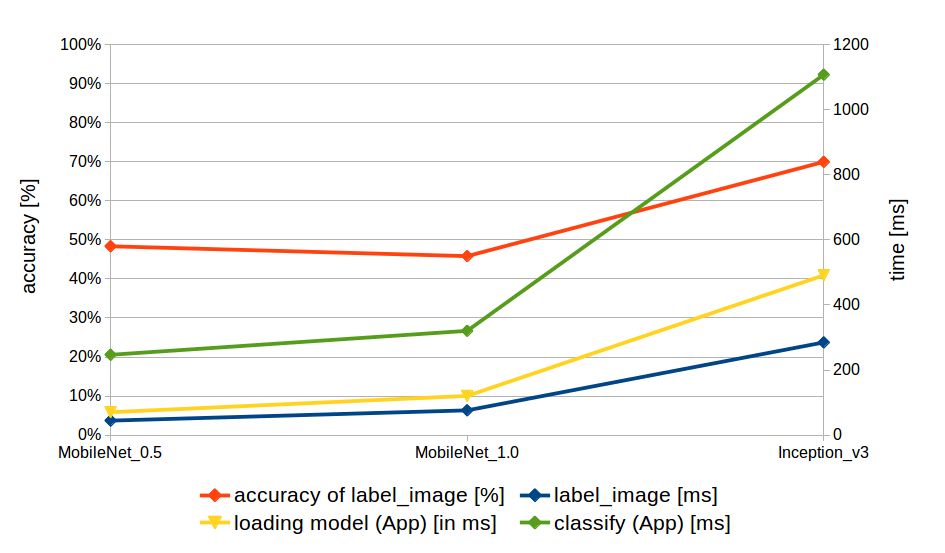
\includegraphics[width=0.9\textwidth]{includes/evalTimesModels}
\caption{Graph for final evaluation of model architecture}
\label{fig:finalEval}
\end{figure}